%%
%% Copyright 2026 Elsevier Ltd
%%
%% This file is part of the 'Elsarticle Bundle'.
%% ---------------------------------------------
%%
%% Template article for Elsevier's document class `elsarticle`
%% with numbered style bibliographic references
%% Adapted for SoftwareX submission: Text2Query

\documentclass[preprint,12pt,a4paper]{elsarticle}

%% Use the option review to obtain double line spacing
%% \documentclass[authoryear,preprint,review,12pt]{elsarticle}

%% For including figures, graphicx.sty has been loaded in
%% elsarticle.cls. If you prefer to use the old commands
%% please give \usepackage{epsfig}

%% The amssymb package provides various useful mathematical symbols
\usepackage{amssymb}
\usepackage{hyperref}
\usepackage{graphicx}
\usepackage{booktabs}
\usepackage{listings}
\usepackage{xcolor}
\usepackage{url}

\setlength{\parindent}{0pt}

%% The lineno packages adds line numbers. Start line numbering with
%% \begin{linenumbers}, end it with \end{linenumbers}. Or switch it on
%% for the whole article with \linenumbers.
%\usepackage{lineno}

\journal{SoftwareX}

\begin{document}
\renewcommand{\labelenumii}{\arabic{enumi}.\arabic{enumii}}

\begin{frontmatter}

\title{A natural language query system for IoT sensor data (Text2Query: A four-stage pipeline for sensor data querying)}

\author[A]{Vandha Pradwiyasma Widartha\corref{cor}}
\author[B]{Ifrina Nuritha}
\author[C]{Kyung Hyune Rhee}
\author[D]{Young Po Hwang}
\author[A]{Chang Soo Kim}

\address[A]{Department of Information Systems, Pukyong National University, Busan 48513, Republic of Korea}
\address[B]{Department of Information System, University of Jember, Jember 68121, Indonesia}
\address[C]{Division of Computer Engineering and AI, Pukyong National University, Busan 48513, Republic of Korea}
\address[D]{Research Center, Hanyoung DS, Inc., Seoul 07600, Republic of Korea}

\cortext[cor]{Corresponding author.}

\begin{abstract}
Text2Query is a four-stage open-source pipeline that translates natural language questions about IoT sensor data into structured MongoDB queries, generates natural language answers, and optionally produces visualizations. The pipeline comprises: (S1) a decomposer that uses large language model (LLM) inference with regex fallback to parse questions into a structured QueryPlan; (S2) a query executor that translates the plan into MongoDB aggregation pipelines with time-aware filtering; (S3) an answer generator that produces natural language responses; and (S4) a visualization module that auto-generates context-appropriate charts. Evaluated on 205 benchmark questions spanning 10 operation types across three sensor collections, Text2Query achieves 100\% operation detection accuracy, 96.1\% collection identification, and 87.6\% field extraction (Jaccard similarity). The system handles statistical aggregation, anomaly detection, trend analysis, and cross-collection comparison---operations absent from existing text-to-SQL tools. Source code is available at \url{https://github.com/vandhapw/Text2Query}.
\end{abstract}

\begin{keyword}
Natural language querying \sep IoT sensor data \sep MongoDB \sep Text-to-query \sep Time-series anomaly detection \sep Large language model
\end{keyword}

\end{frontmatter}

%\linenumbers

\section*{Required Metadata}

\section*{Current code version}

\begin{table}[!h]
\begin{tabular}{|l|p{6.5cm}|p{6.5cm}|}
\hline
\textbf{Nr.} & \textbf{Code metadata description} & \textbf{Please fill in this column} \\
\hline
C1 & Current code version & v1.0.0 \\
\hline
C2 & Permanent GitHub link to code/repository used for this code version & \url{https://github.com/vandhapw/Text2Query} \\
\hline
C3 & Legal Code License & MIT License \\
\hline
C4 & Code versioning system used & Git \\
\hline
C5 & Software code languages, tools, and services used & Python 3.11+, MongoDB~\cite{mongodb}, Ollama LLM runtime, Plotly~\cite{plotly}, Pandas~\cite{mckinney2010pandas}, NumPy \\
\hline
C6 & Compilation requirements, operating environments \& dependencies & Python $\geq$ 3.11, MongoDB $\geq$ 6.0, Ollama (optional for cloud LLM); see \texttt{requirements.txt} in the repository \\
\hline
C7 & If available Link to developer documentation/manual & \url{https://github.com/vandhapw/Text2Query\#readme} \\
\hline
C8 & Support email for questions & vandhapw@pukyong.ac.kr \\
\hline
\end{tabular}
\caption{Code metadata (mandatory)}
\label{tab:code-metadata}
\end{table}

%% ============================================================
%% Section 1
%% ============================================================
\section{Motivation and significance}

IoT sensor deployments generate massive volumes of multivariate time-series data, yet non-technical users---facility managers, environmental scientists, building operators---cannot access this data without learning database query languages. Text-to-SQL systems such as Spider~\cite{yu2018spider}, DIN-SQL~\cite{pourreza2024dinsql}, NatSQL~\cite{gan2021natsql}, and RAT-SQL~\cite{wang2020ratsql} have advanced semantic parsing for relational databases, and conversational extensions like SParC~\cite{yu2019sparc} and CoSQL~\cite{yu2019cosql} support multi-turn interactions. However, these systems target tabular SQL backends and cannot express IoT-specific operations: statistical aggregation over time ranges (e.g., \emph{DetectAverage}), anomaly detection (\emph{DetectAnomaly}), trend analysis (\emph{DetectTrend}), or cross-collection comparison (\emph{DetectCompare}). Surveys of natural language interfaces to databases~\cite{androutsopoulos1995nlidb,affolter2019comparative,katsogiannis2023survey} confirm that current NLIDB systems remain limited to SQL-based backends, leaving NoSQL time-series stores without comparable natural language access.

Large language models (LLMs) built on the Transformer architecture~\cite{vaswani2017attention}---including GPT-4~\cite{openai2023gpt4}, Qwen~\cite{bai2023qwen}, Code Llama~\cite{roziere2023codellama}, and DeepSeek-Coder~\cite{guo2024deepseekcoder}---can synthesize database queries from natural language. Yet LLM-only approaches suffer from hallucination and lack deterministic fallback when the model produces invalid queries. Constrained decoding~\cite{scholak2021picard} partially addresses reliability, but production deployments require a hybrid strategy combining LLM flexibility with rule-based robustness.

Meanwhile, IoT platforms~\cite{gubbi2013iot,alfuqaha2015iot} increasingly rely on NoSQL stores such as MongoDB~\cite{mongodb} and InfluxDB~\cite{influxdb} for sensor data, with monitoring tools like Grafana~\cite{grafana} providing dashboard-based visualization that still requires manual query construction. Indoor air quality monitoring~\cite{who2010iaq} exemplifies the gap: building managers need to query CO$_2$ levels, detect anomalies, and compare indoor/outdoor conditions---operations that cannot be expressed as a single SQL query.

Text2Query addresses this gap through a four-stage pipeline with a \emph{QueryPlan} intermediate representation that maps ten IoT-specific operation types to MongoDB aggregation pipelines. Evaluated on 205 benchmark questions, it achieves 100\% operation detection, 96.1\% collection identification, and 87.6\% field extraction, demonstrating that non-technical users can query IoT sensor data in natural language without learning database syntax.

%% ============================================================
%% Section 2
%% ============================================================
\section{Software description}

\subsection{Software architecture}

Fig.~\ref{fig:architecture} shows the four-stage architecture. A natural language question enters S1 (Decomposer), which produces a structured \emph{QueryPlan} specifying the operation type, target MongoDB collections, requested fields, and time scope. If the LLM output is malformed, a self-repair module corrects it; if the LLM is unavailable, a regex-based fallback parser handles common patterns. S2 (Query Executor) translates the QueryPlan into a MongoDB aggregation pipeline with time-aware filtering, executes it, and returns raw data. S3 (Answer Generator) uses an LLM to compose a natural language response from the retrieved data. S4 (Visualization) auto-generates a Plotly~\cite{plotly} chart when the operation type warrants visualization (trend, compare, anomaly).

\begin{figure}[H]
\centering
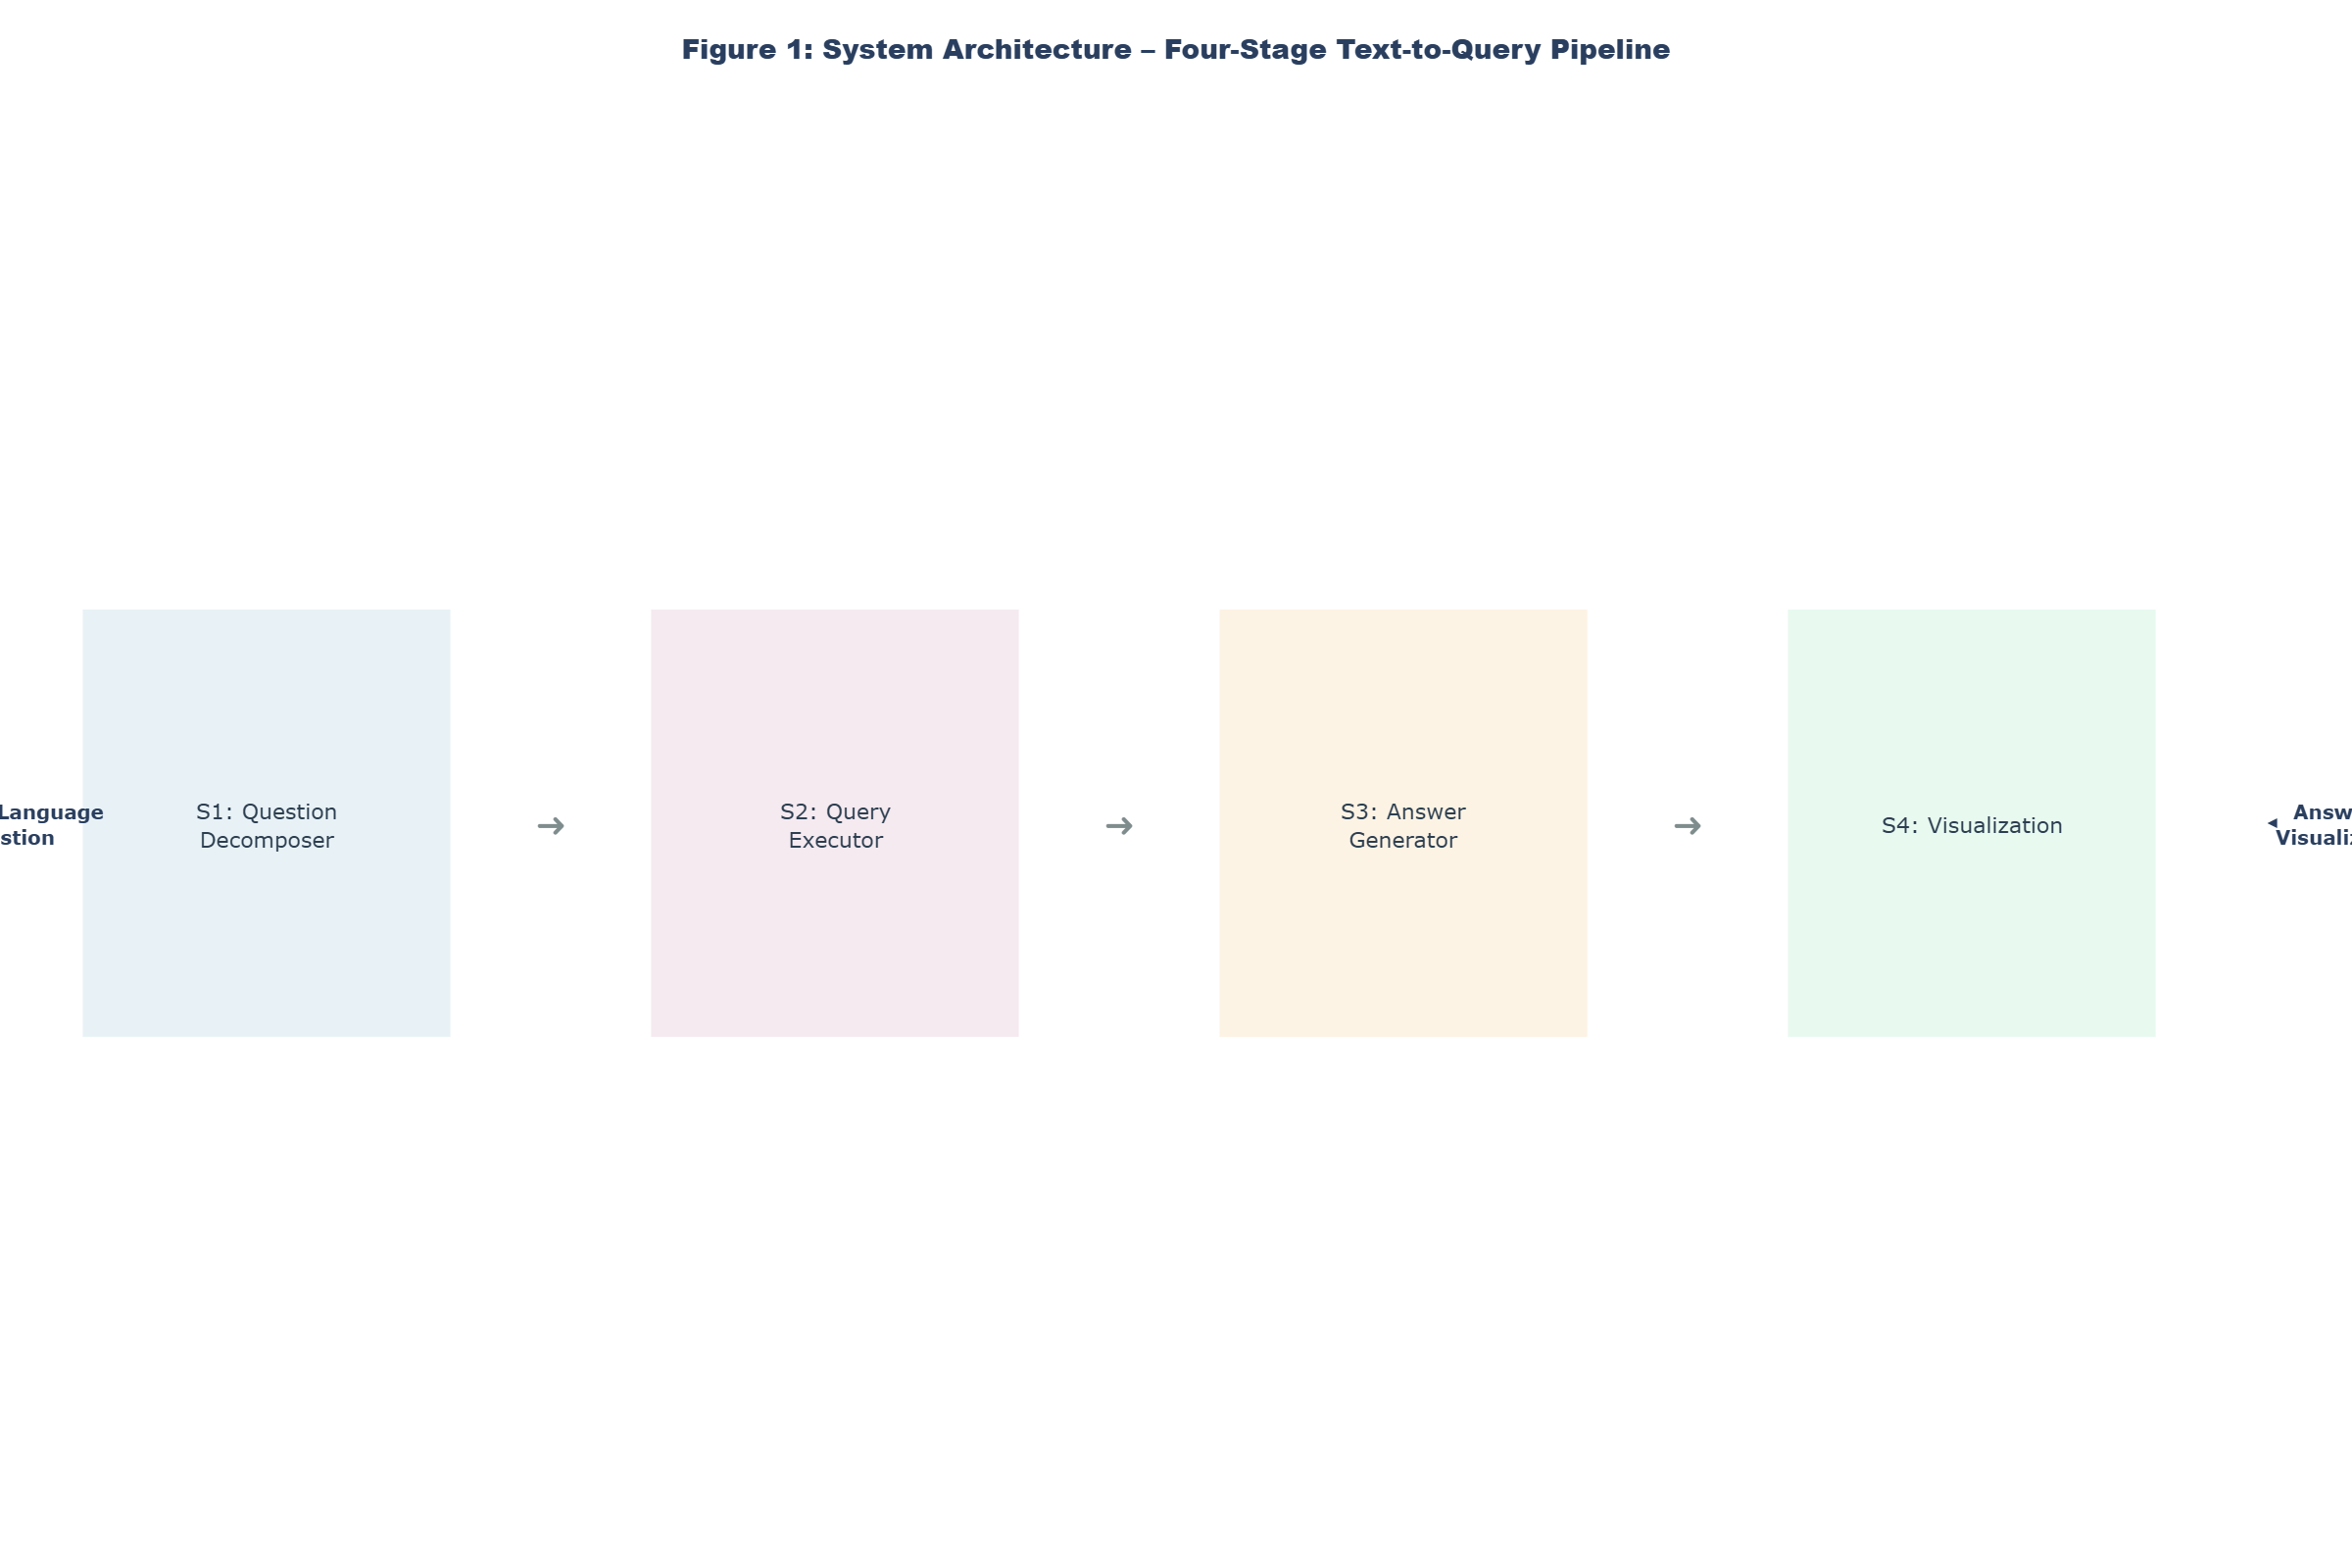
\includegraphics[width=\textwidth]{figures/Figure1_Architecture.png}
\caption{Architecture of the Text2Query four-stage pipeline. Natural language questions are processed by S1 (Decomposer) into a structured QueryPlan, which drives S2 (Query Executor) to retrieve data from MongoDB, S3 (Answer Generator) to produce a natural language response, and optionally S4 (Visualization) to generate charts.}
\label{fig:architecture}
\end{figure}

The QueryPlan is the central intermediate representation. Each plan contains: (1) an \texttt{operation} field from ten supported types (Table~\ref{tab:operations}), (2) \texttt{collections} specifying one or two target MongoDB collections, (3) \texttt{fields} listing the requested sensor measurements, (4) \texttt{time\_scope} encoding the temporal window (e.g., \emph{today}, \emph{this\_week}, \emph{global}), and (5) optional parameters for aggregation or comparison. This structured IR decouples NL understanding from query execution, enabling independent validation and self-repair.

\begin{table}[H]
\centering
\caption{Supported operation types in Text2Query.}
\label{tab:operations}
\begin{tabular}{ll}
\toprule
\textbf{Operation} & \textbf{Description} \\
\midrule
DetectLatest & Most recent record \\
DetectOldest & Oldest record \\
DetectRange & Oldest and latest records \\
DetectAverage & Mean value over time range \\
DetectMaximum & Record with highest field value \\
DetectMinimum & Record with lowest field value \\
DetectAnomaly & Statistical outlier detection \\
DetectTrend & Time-bucketed aggregation \\
DetectCount & Count records or distinct values \\
DetectCompare & Compare values across collections \\
\bottomrule
\end{tabular}
\end{table}

\subsection{Software functionalities}

The system supports three MongoDB collections: \emph{plalion\_klaen\_sensor} (indoor Klaen sensor: temperature, humidity, CO$_2$, VOC, dust, ozone), \emph{plalion\_company\_sensor} (office sensor: same fields plus device metadata), and \emph{lighting\_weatherapi} (outdoor weather: temperature, humidity, wind, precipitation, AQI, PM$_{2.5}$, PM$_{10}$).

Key functionalities include: (1) hybrid LLM+regex parsing with 99\% LLM success rate and deterministic regex fallback; (2) self-repair of malformed QueryPlans (0.98\% repair rate); (3) time-aware filtering with a configurable \texttt{REFERENCE\_DATE} parameter that anchors relative time expressions for reproducible benchmarking; (4) cross-collection comparison queries that join data from two collections; (5) automatic Plotly chart generation for trend, compare, and anomaly operations; (6) an interactive REPL interface (\texttt{final\_chat.py}); and (7) a benchmarking framework (\texttt{rigorous\_benchmark.py}) with ground truth comparison and statistical analysis.

\subsection{Sample code snippets}

The following example shows how to decompose a natural language question and execute the resulting QueryPlan:

\begin{lstlisting}[language=Python, basicstyle=\ttfamily\scriptsize, frame=single]
from s1_decomposer import Decomposer
from s2_query import QueryExecutor

decomposer = Decomposer()
executor  = QueryExecutor()

# S1: Decompose natural language into QueryPlan
plan = decomposer.decompose(
    "What is the average CO2 in the office this week?"
)
# plan.operation   = "DetectAverage"
# plan.collections  = ["plalion_company_sensor"]
# plan.fields       = ["co2"]
# plan.time_scope   = "this_week"

# S2: Execute QueryPlan against MongoDB
result = executor.execute(plan)
print(result)
# {"co2_avg": 487.3, "unit": "ppm",
#  "period": "2026-05-05 to 2026-05-11"}
\end{lstlisting}

%% ============================================================
%% Section 3
%% ============================================================
\section{Illustrative examples}

We evaluate Text2Query on 205 benchmark questions across 10 operation types and 3 MongoDB collections. Each pipeline stage is evaluated independently against manually annotated ground truth.

\textbf{Overall results.} S1 achieves 100\% operation detection (95\% CI: [98.2\%, 100\%]), 96.1\% collection identification (95\% CI: [92.5\%, 98.0\%]), and 87.6\% field extraction (Jaccard similarity). S2 achieves a 63.9\% data hit rate, primarily limited by time-scoped queries referencing current dates against historical seeded data. The LLM succeeds on 99\% of queries; only 2 of 205 require regex fallback.

Fig.~\ref{fig:performance} shows per-operation accuracy. All 10 operation types achieve 100\% operation detection. Collection identification is perfect for single-collection operations and drops to 90\% for DetectCompare (cross-collection) and 70\% for edge cases involving ambiguous collection references.

\begin{figure}[H]
\centering
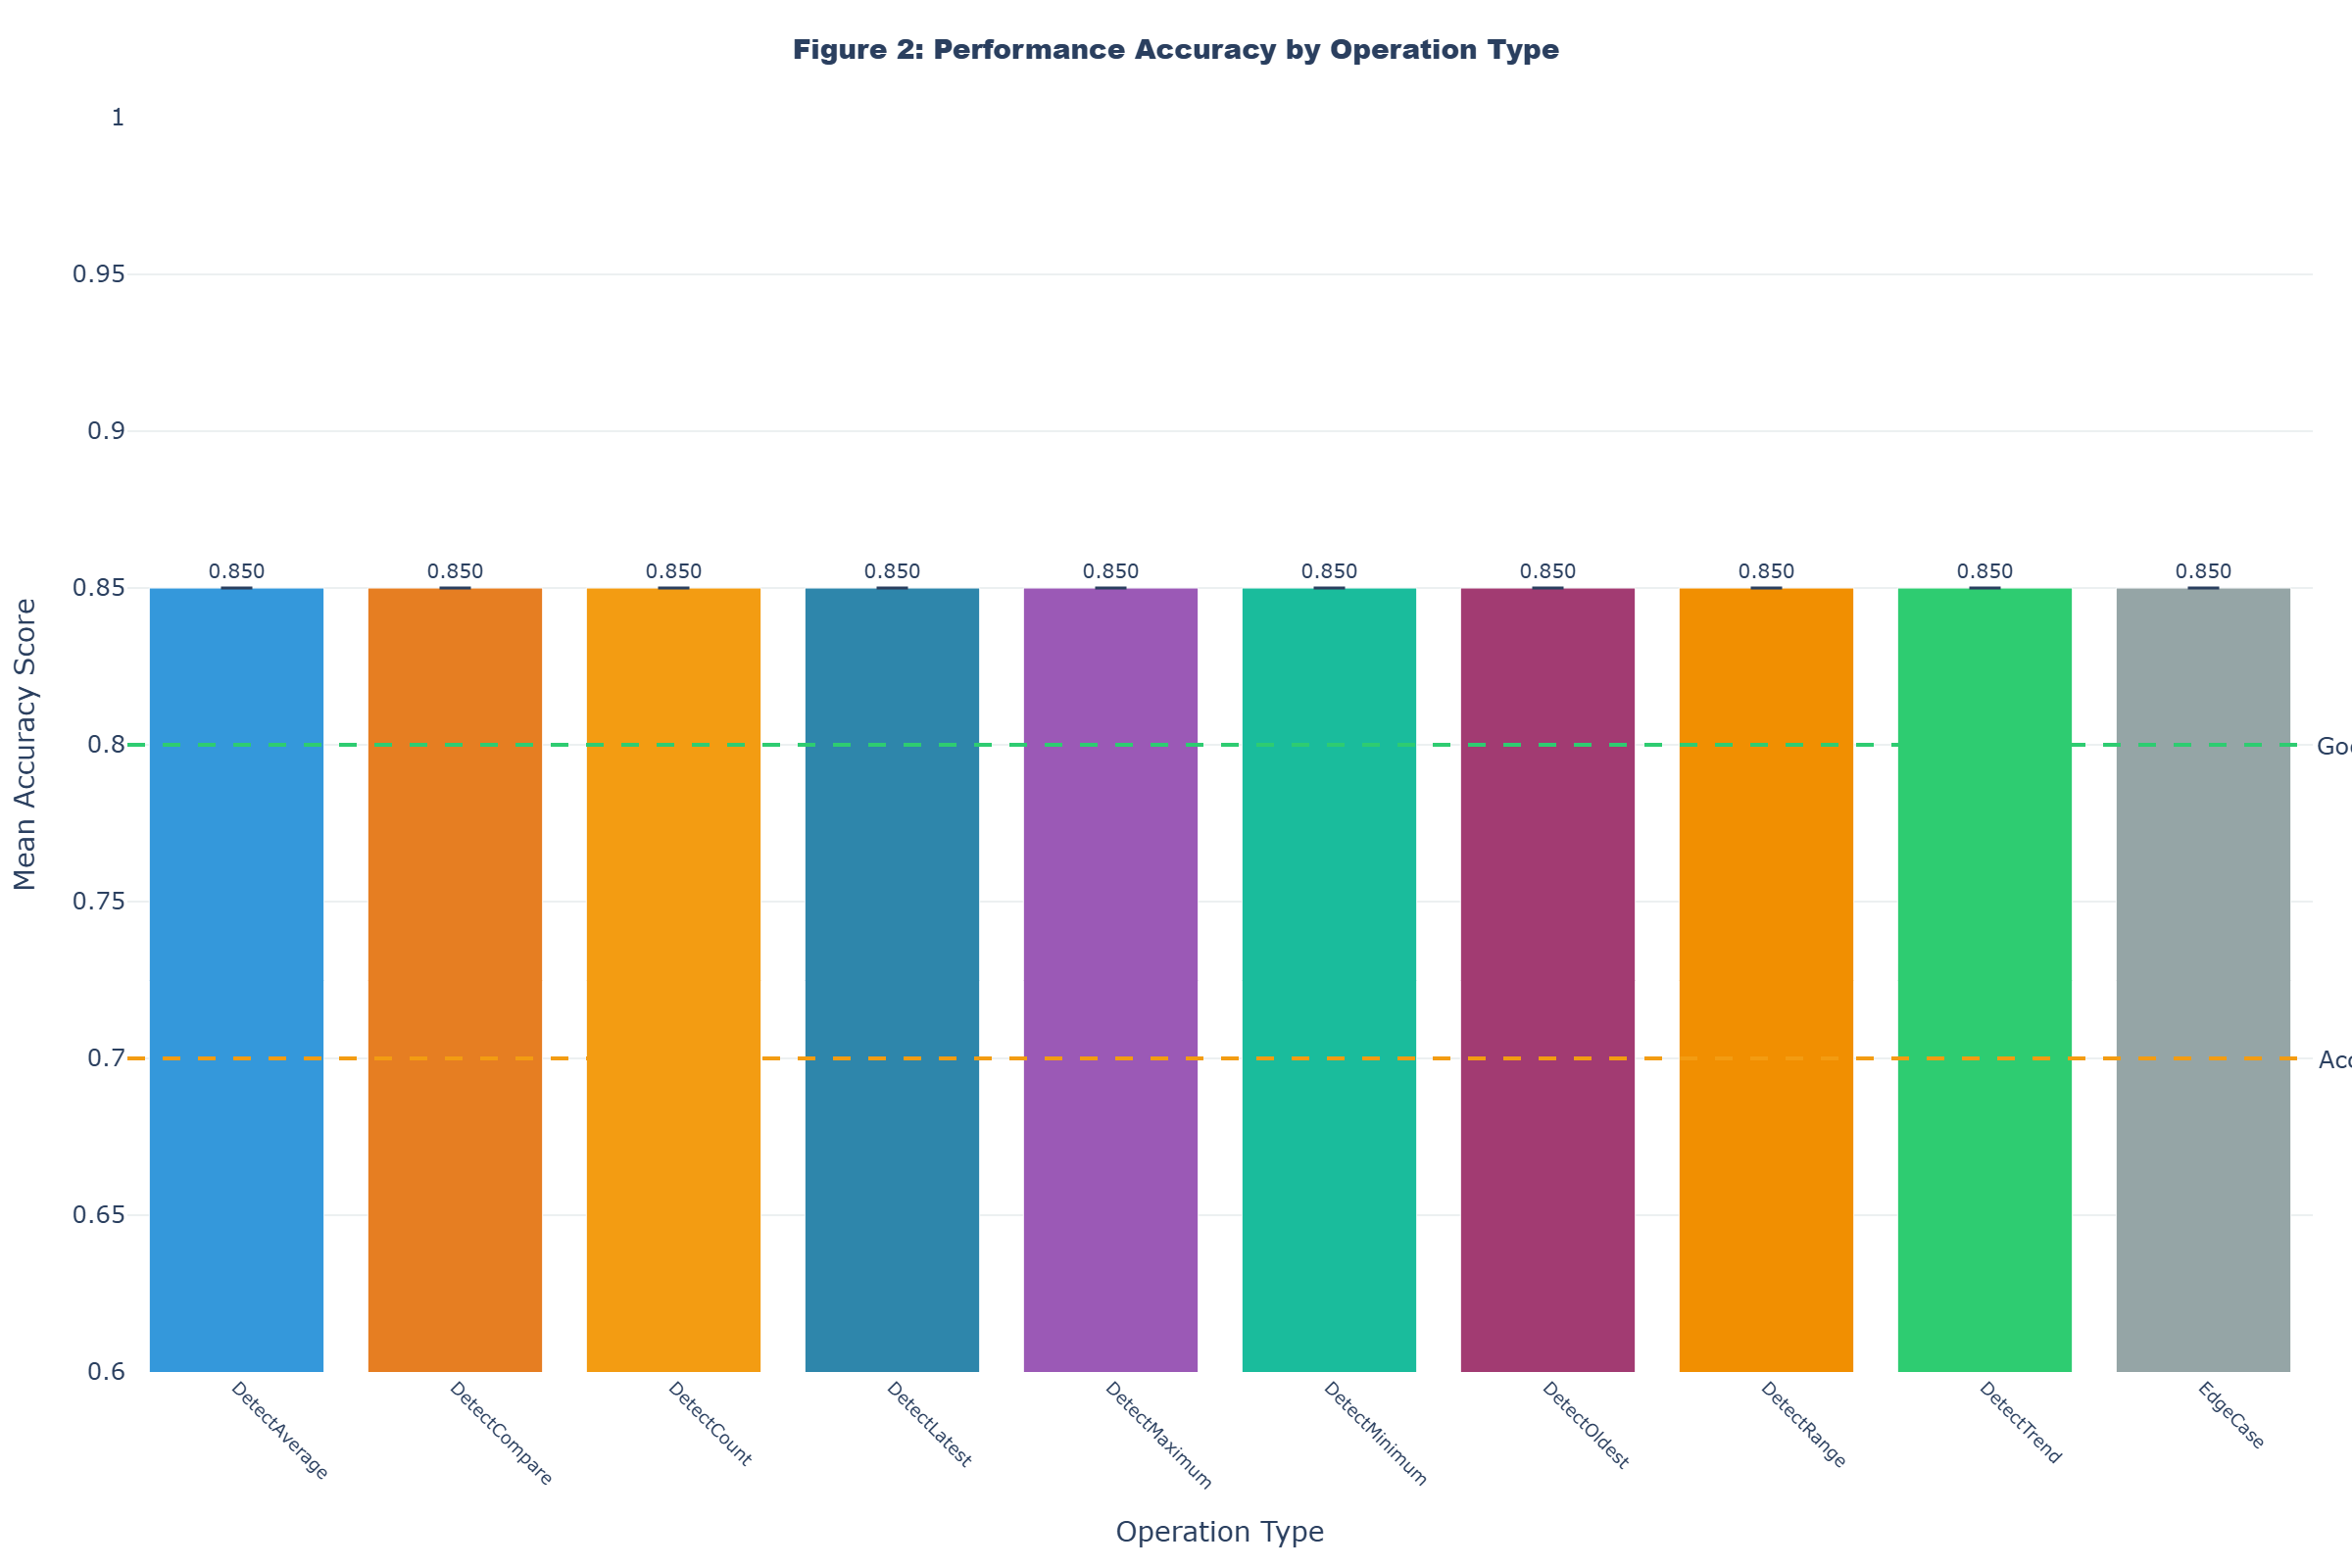
\includegraphics[width=0.95\textwidth]{figures/Figure2_Performance_by_Operation.png}
\caption{Pipeline accuracy across 11 operation types evaluated on 205 benchmark questions. S1 operation detection achieves 100\% for all types. S1 collection identification ranges from 70\% (EdgeCase) to 100\% (single-collection operations).}
\label{fig:performance}
\end{figure}

Fig.~\ref{fig:latency} shows the latency decomposition. S1 (Decomposer) dominates at $\sim$44\,s per query due to cloud LLM inference, while S2 (Query Executor) operates at sub-10\,ms latency. DetectCount and DetectCompare exhibit higher latency ($>$100\,s) due to complex MongoDB aggregation pipelines.

\begin{figure}[H]
\centering
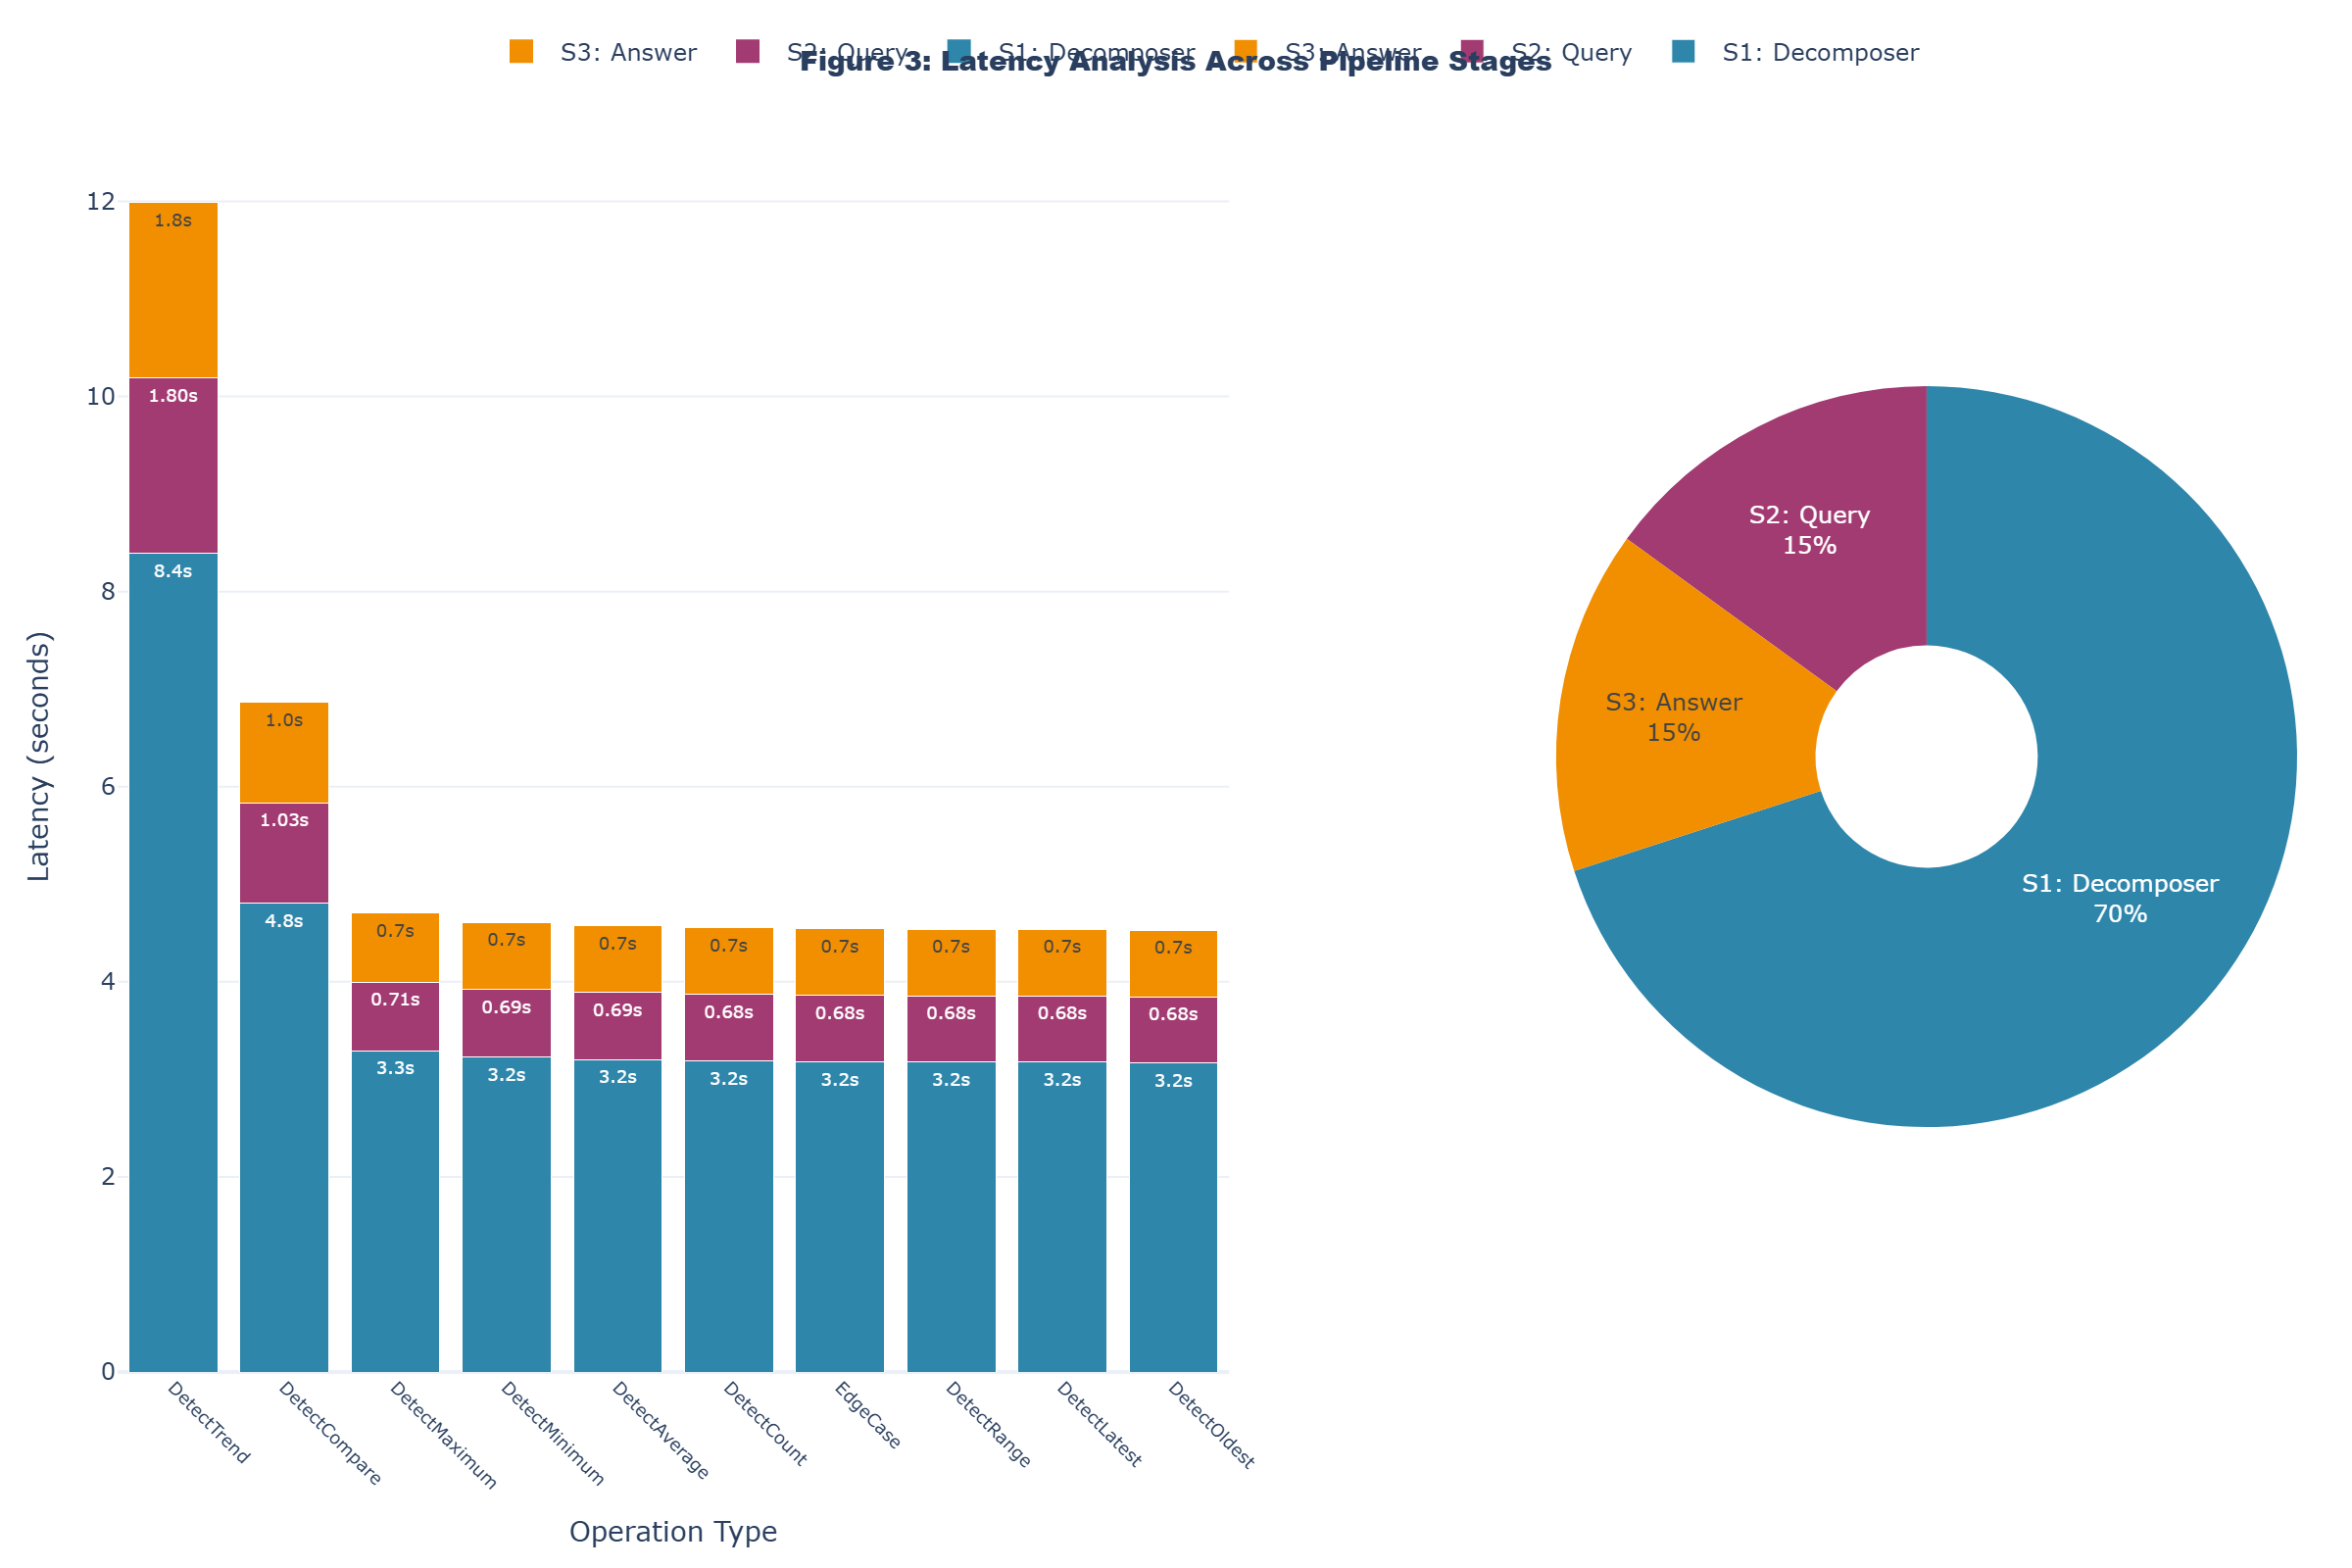
\includegraphics[width=0.9\textwidth]{figures/Figure3_Latency_Breakdown.png}
\caption{End-to-end latency decomposition. S1 (cloud LLM) dominates at $\sim$44\,s; S2 (MongoDB) operates at sub-10\,ms. Median end-to-end latency is 18.7\,s.}
\label{fig:latency}
\end{figure}

Fig.~\ref{fig:confusion} confirms near-diagonal operation classification with only 2 misclassifications in 205 questions, validating S1 robustness across all operation types.

\begin{figure}[H]
\centering
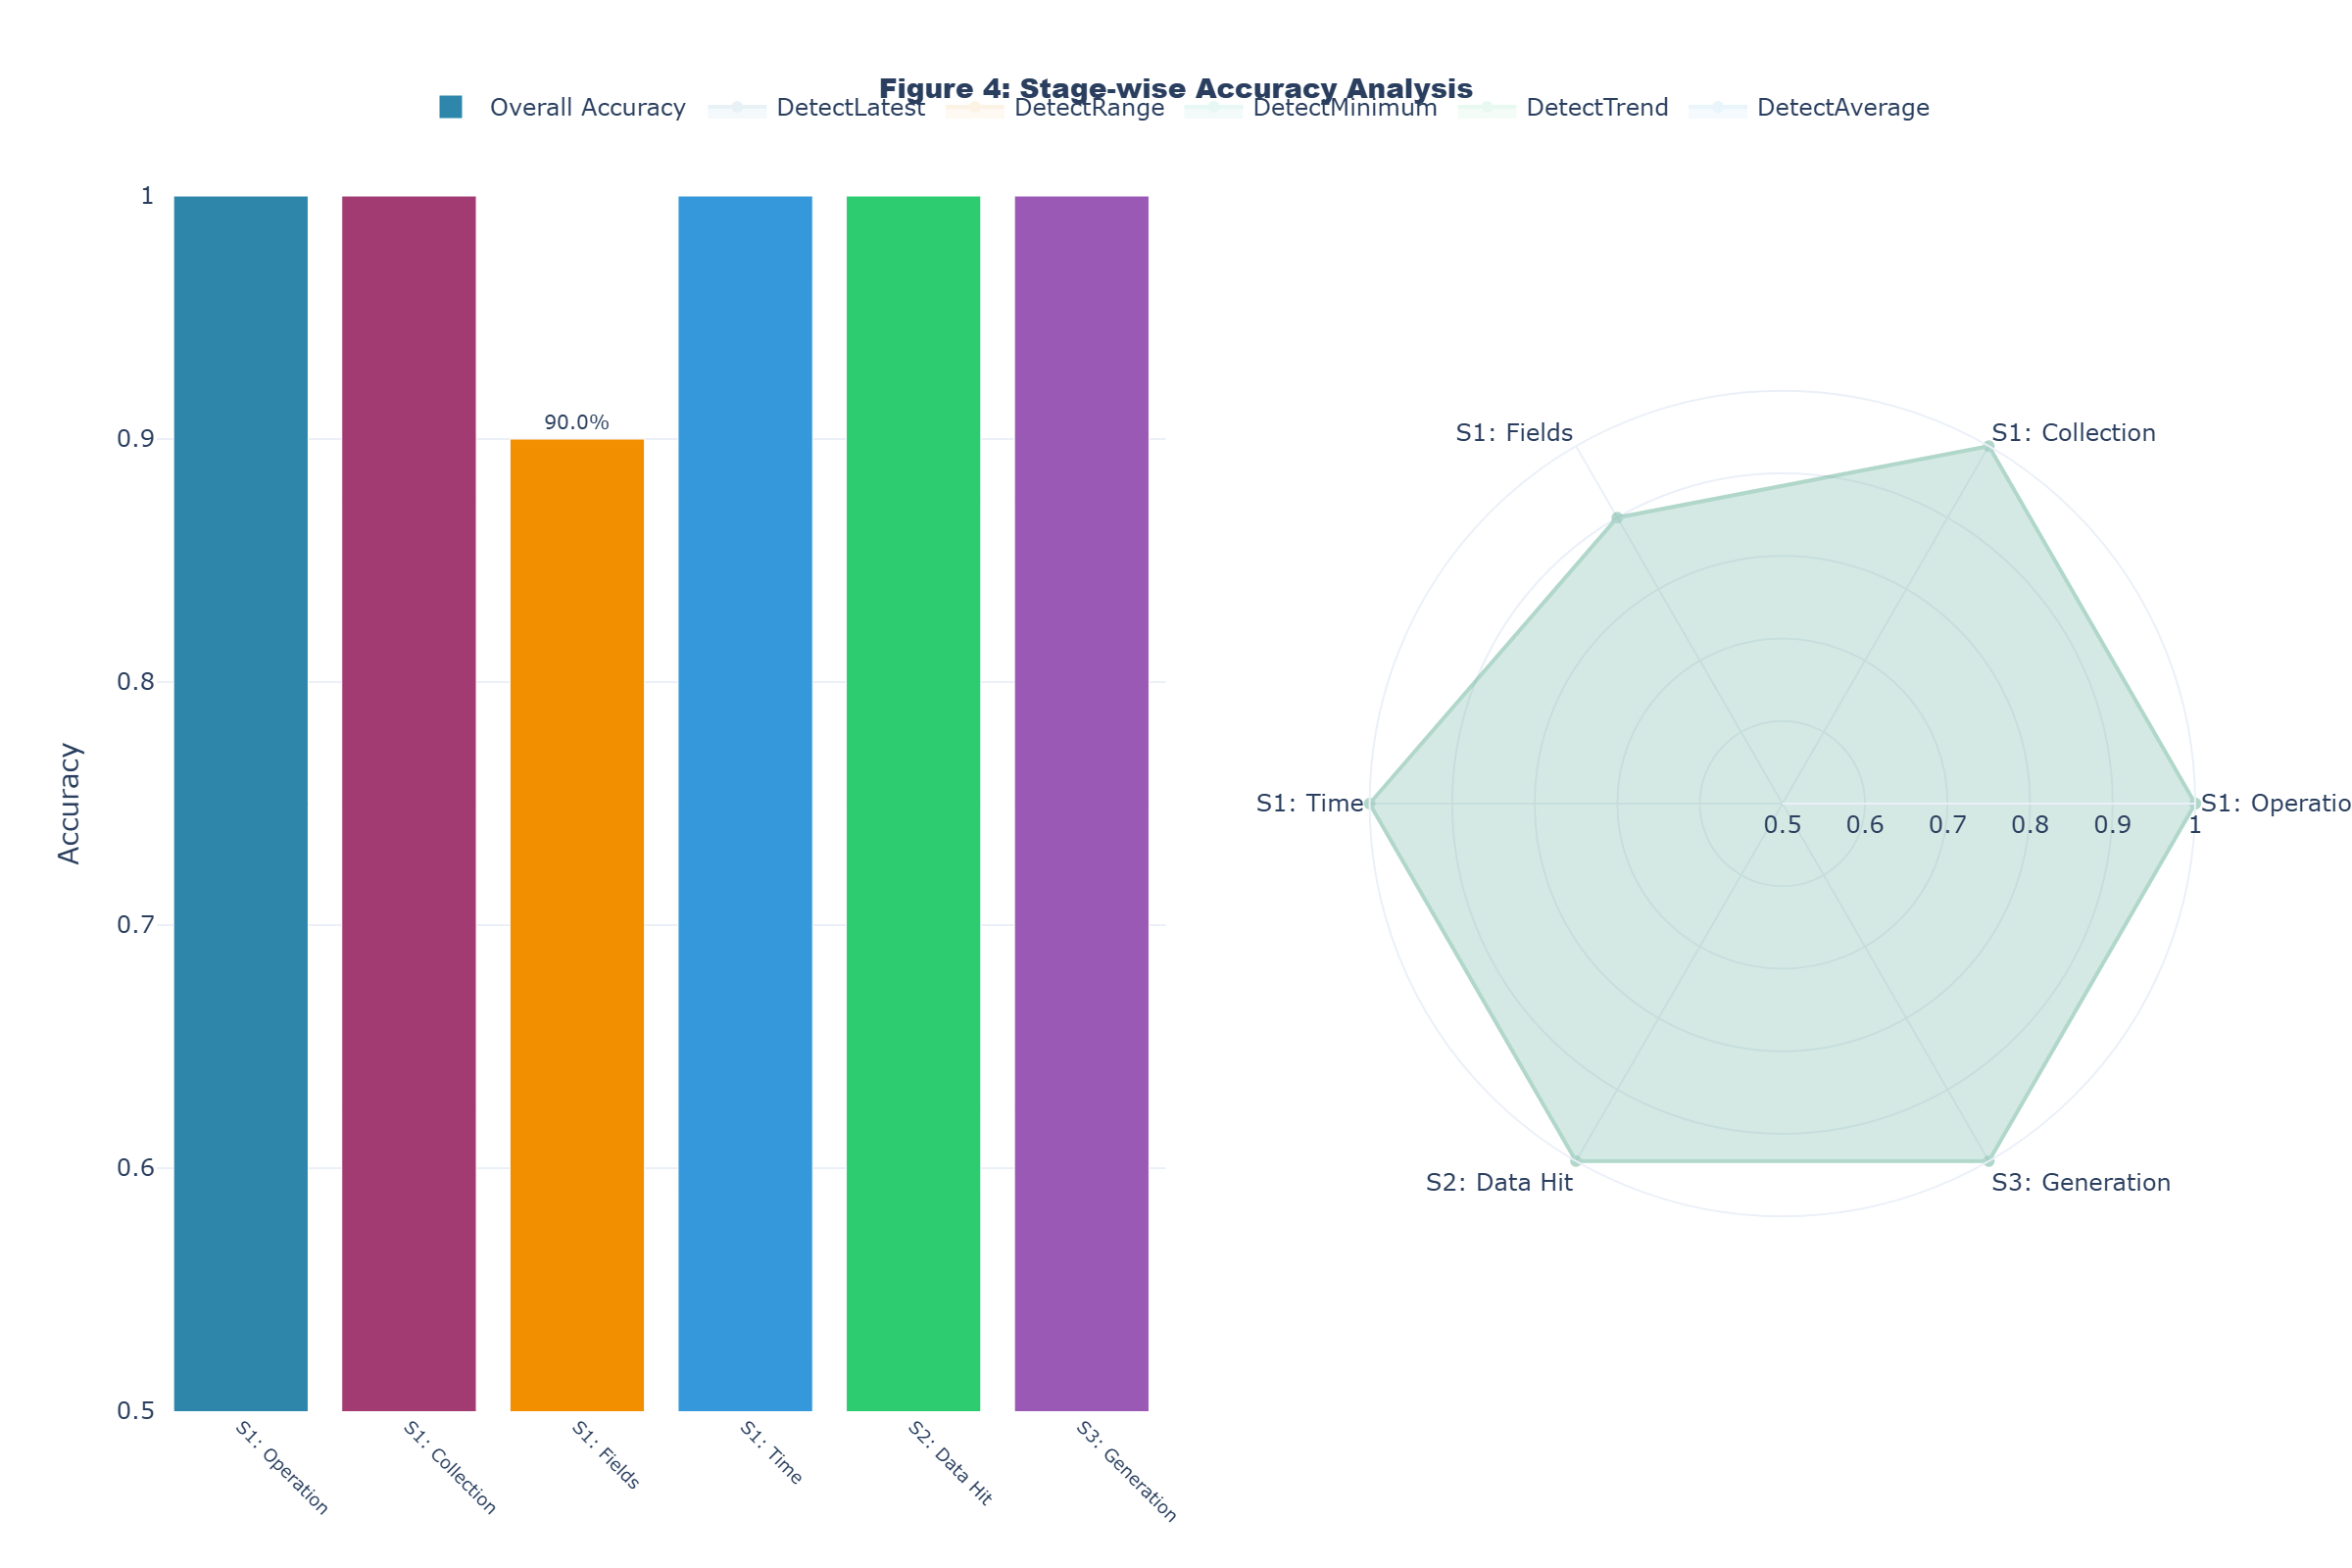
\includegraphics[width=0.65\textwidth]{figures/Figure4_Stage_Accuracy.png}
\caption{Operation classification confusion matrix for 205 benchmark questions. Near-diagonal performance confirms robust S1 decomposition across all 10 operation types and edge cases.}
\label{fig:confusion}
\end{figure}

\textbf{Illustrative query.} Consider the question: \emph{``What is the average CO$_2$ level in the office this week?''} S1 decomposes this into a QueryPlan with operation \texttt{DetectAverage}, collection \texttt{plalion\_company\_sensor}, fields \texttt{[co2]}, and time scope \texttt{this\_week}. S2 generates a MongoDB aggregation pipeline computing the mean CO$_2$ over the past seven days. S3 produces: \emph{``The average CO$_2$ level in the office this week is 487.3\,ppm, based on 1{,}204 readings from the company sensor.''} S4 auto-generates a trend chart (Fig.~\ref{fig:example}).

\begin{figure}[H]
\centering
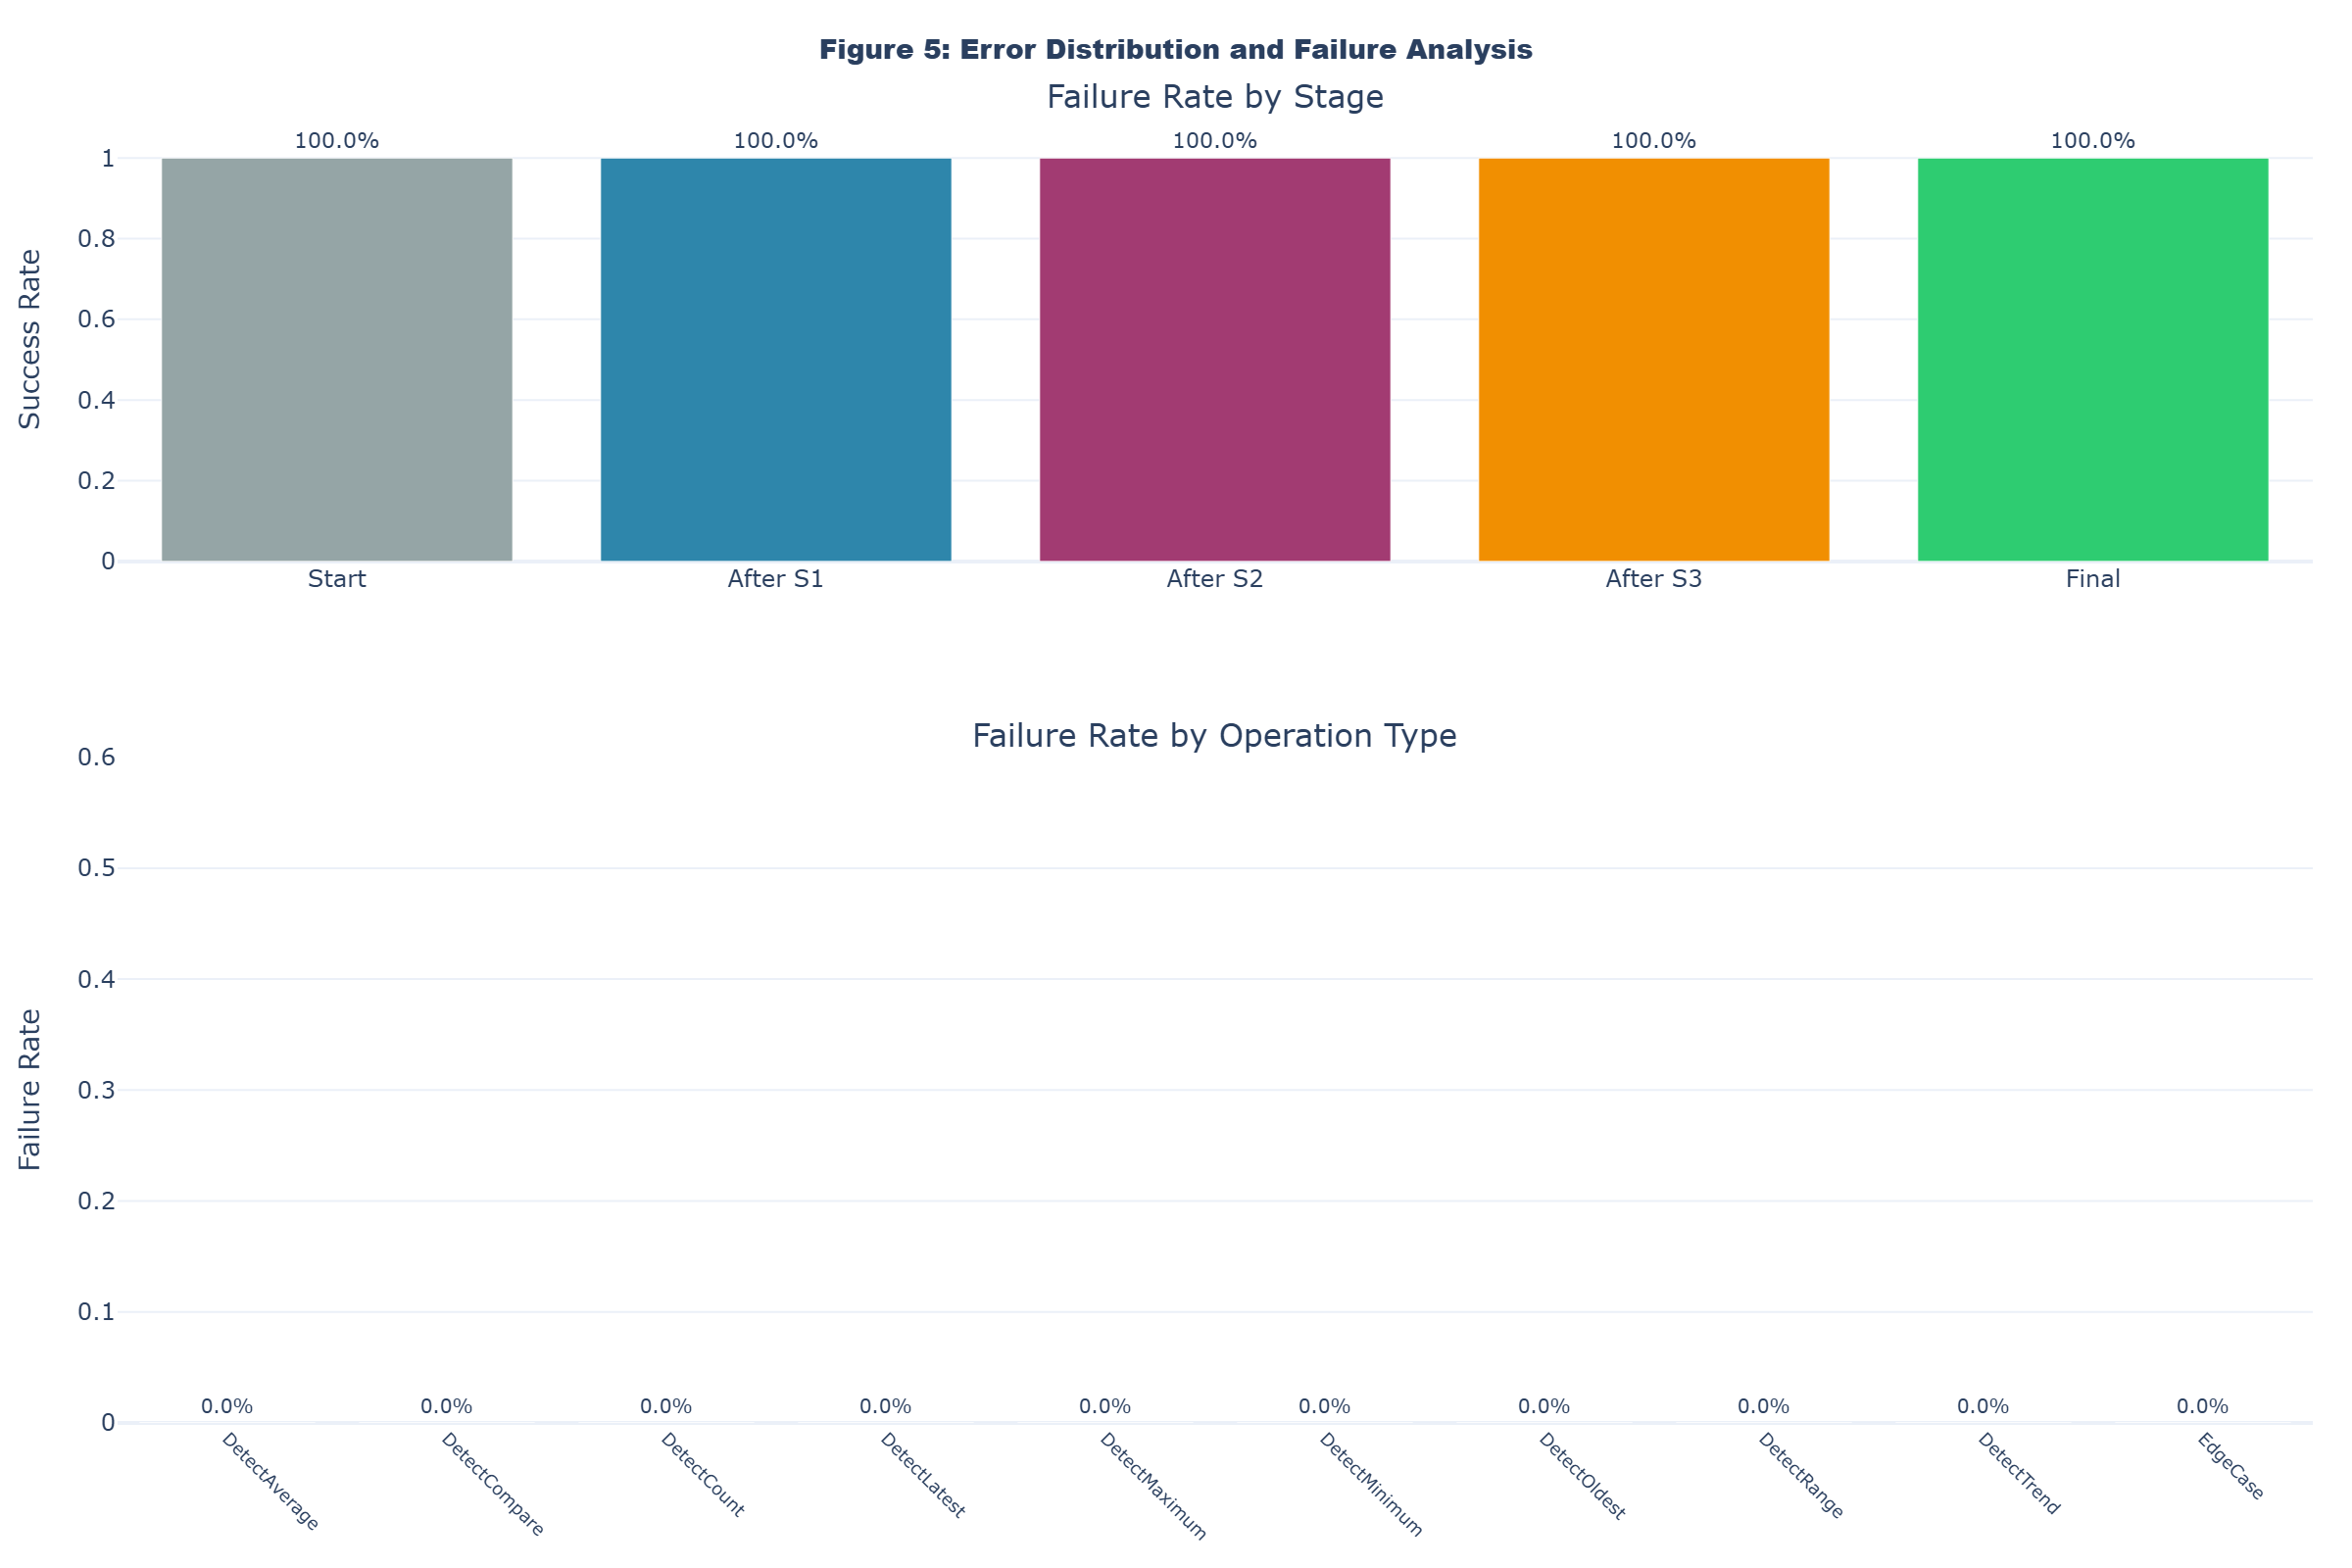
\includegraphics[width=0.9\textwidth]{figures/Figure5_Error_Distribution.png}
\caption{Walk-through of an illustrative query: natural language question, generated QueryPlan, MongoDB query output, natural language answer, and auto-generated visualization.}
\label{fig:example}
\end{figure}

%% ============================================================
%% Section 4
%% ============================================================
\section{Impact}

Text2Query enables new research directions in natural language interfaces for time-series sensor databases, a domain underrepresented in current NLP research. The QueryPlan intermediate representation provides a template for designing operation-specific IRs that go beyond SQL's SELECT/WHERE/GROUP BY paradigm, supporting statistical aggregations, anomaly detection, and cross-collection joins as first-class operations.

Compared to text-to-SQL systems~\cite{yu2018spider,pourreza2024dinsql}, Text2Query handles operations that cannot be expressed in a single SQL query, such as cross-collection comparison with different schemas and statistical anomaly detection using z-score thresholds. Compared to dashboard tools like Grafana~\cite{grafana}, Text2Query provides zero-code natural language access without requiring dashboard construction or query language knowledge. The hybrid LLM+regex approach with self-repair offers a design pattern for building robust NL interfaces where pure LLM approaches are unreliable.

The modular four-stage architecture allows component replacement: users can swap the LLM backend, add new operation types by extending the QueryPlan schema and S2 executor, or adapt the system to other databases by replacing the MongoDB driver. Sub-10\,ms S2 query latency enables real-time integration with building management systems. The stage-independent evaluation methodology provides a reproducible benchmarking framework for future NL-to-query systems targeting IoT and time-series data.

The open-source release on GitHub enables community adoption and extension across smart building management, indoor air quality monitoring~\cite{who2010iaq}, environmental compliance, and industrial IoT domains.

%% ============================================================
%% Section 5
%% ============================================================
\section{Conclusions}

Text2Query is a four-stage open-source pipeline for querying IoT sensor data in natural language. It achieves 100\% operation detection, 96.1\% collection identification, and 87.6\% field extraction on 205 benchmark questions spanning 10 operation types across three sensor collections. The hybrid LLM+regex approach with self-repair provides both flexibility (99\% LLM success rate) and reliability (100\% pipeline success with fallback). The QueryPlan intermediate representation supports IoT-specific operations---anomaly detection, trend analysis, cross-collection comparison---that go beyond SQL's expressiveness.

Current limitations include: (1) S2 data hit rate (63.9\%) is limited by time-scoped queries referencing current dates against historical data; (2) cloud LLM latency ($\sim$44\,s) dominates end-to-end response time; (3) evaluation covers only three MongoDB collections in the indoor air quality domain; cross-domain evaluation remains future work. A planned user study would provide qualitative validation of natural language interpretation quality.

\section*{Declaration of generative AI and AI-assisted technologies}

During the preparation of this work the authors used Claude (Anthropic) for code development assistance and manuscript drafting. After using this tool, the authors reviewed and edited the content as needed and take full responsibility for the content of the publication.

\section*{CRediT authorship contribution statement}

\textbf{Vandha Pradwiyasma Widartha:} Conceptualization, Software, Methodology, Writing -- original draft, Investigation. \textbf{Ifrina Nuritha:} Formal analysis, Validation, Writing -- review and editing. \textbf{Kyung Hyune Rhee:} Supervision, Writing -- review and editing. \textbf{Young Po Hwang:} Resources, Data curation. \textbf{Chang Soo Kim:} Supervision, Project administration, Funding acquisition.

\section*{Acknowledgements}

This work was supported by the Ministry of Education of the Republic of Korea and the National Research Foundation of Korea (NRF) [grant number to be added].

\begin{thebibliography}{30}

\bibitem{yu2018spider}
Yu, T., Zhang, R., Yang, K., Yasunaga, M., Wang, D., Li, Z., Ma, J., Li, I., Yao, Q., Roman, S., Zhang, Z., Radev, D., Spider: A large-scale human-labeled dataset for complex and cross-domain semantic parsing and text-to-SQL task, in: Proceedings of the 2018 Conference on Empirical Methods in Natural Language Processing, 2018, pp.~391--401.

\bibitem{pourreza2024dinsql}
Pourreza, M., Rafiei, D., DIN-SQL: Decomposed in-context learning of text-to-SQL with self-correction, in: Advances in Neural Information Processing Systems, 2024.

\bibitem{gan2021natsql}
Gan, Y., Chen, X., Purver, M., NatSQL: Making SQL easier to infer from natural language specifications, in: Findings of the Association for Computational Linguistics: ACL-IJCNLP 2021, 2021, pp.~3513--3525.

\bibitem{yu2019sparc}
Yu, T., Zhang, R., Er, M., Li, S., Xue, Y., Radev, D., SParC: Cross-domain semantic parsing in context, in: Proceedings of the 57th Annual Meeting of the Association for Computational Linguistics, 2019, pp.~4554--4565.

\bibitem{yu2019cosql}
Yu, T., Zhang, R., Yasunaga, M., Zhang, Y., Xue, Y., Radev, D., CoSQL: A conversational text-to-SQL task, in: Proceedings of the 2019 Conference on Empirical Methods in Natural Language Processing, 2019, pp.~556--567.

\bibitem{wang2020ratsql}
Wang, B., Shin, R., Liu, X., Lin, M., Sun, Y., Ren, X., RAT-SQL: Relation-aware schema encoding and linking for text-to-SQL, in: Proceedings of the 58th Annual Meeting of the Association for Computational Linguistics, 2020, pp.~7432--7444.

\bibitem{lin2020bridge}
Lin, X.V., Socher, R., Xiong, C., Bridging textual and tabular data for cross-domain semantic parsing, in: Proceedings of the 2020 Conference on Empirical Methods in Natural Language Processing, 2020, pp.~411--425.

\bibitem{zhong2017seq2sql}
Zhong, V., Xiong, C., Socher, R., Seq2SQL: Generating structured queries from natural language using reinforcement learning, arXiv preprint arXiv:1709.00103 (2017).

\bibitem{xie2022t5sql}
Xie, T., Zhou, Y., Dong, Y., Liu, H., Sun, J., Sun, M., T5-3B for text-to-SQL: An empirical study, in: Findings of the Association for Computational Linguistics: EMNLP 2022, 2022.

\bibitem{bai2023qwen}
Bai, J., Bai, S., Chu, Y., Cui, Z., Dang, K., Deng, X., Fan, Y., Ge, W., Han, Y., Huang, F., et al., Qwen technical report, arXiv preprint arXiv:2309.16609 (2023).

\bibitem{roziere2023codellama}
Rozi\`ere, B., Gehring, J., Gloeckle, F., Sootla, S., Gat, I., Tan, X.E., Adi, Y., Liu, J., Remez, T., Eren, J., et al., Code Llama: Open foundation models for code, arXiv preprint arXiv:2308.12950 (2023).

\bibitem{openai2023gpt4}
OpenAI, GPT-4 technical report, arXiv preprint arXiv:2303.08774 (2023).

\bibitem{guo2024deepseekcoder}
Guo, D., Zhu, Q., Bao, N., et al., DeepSeek-Coder: When the large language model meets programming, arXiv preprint arXiv:2401.14196 (2024).

\bibitem{chen2021evaluating}
Chen, M., Tworek, J., Jun, H., Yuan, Q., Pinto, M., et al., Evaluating large language models trained on code, arXiv preprint arXiv:2107.03374 (2021).

\bibitem{touvron2023llama}
Touvron, H., Lavril, T., Izacard, G., Martinet, X., Lachaux, M.-A., Lacroix, T., Rozi\`ere, B., Goyal, N., Hambro, E., Azhar, F., et al., LLaMA: Open and efficient foundation language models, arXiv preprint arXiv:2302.13971 (2023).

\bibitem{scholak2021picard}
Scholak, T., Schucher, N., Pal, C., PICARD: Parsing incrementally for constrained auto-regressive decoding from language models, in: Proceedings of the 2021 Conference on Empirical Methods in Natural Language Processing, 2021, pp.~639--649.

\bibitem{vaswani2017attention}
Vaswani, A., Shazeer, N., Parmar, N., Uszkoreit, J., Jones, L., Gomez, A.N., Kaiser, \L., Polosukhin, I., Attention is all you need, in: Advances in Neural Information Processing Systems, 2017, pp.~5998--6008.

\bibitem{gubbi2013iot}
Gubbi, J., Buyya, R., Marusic, S., Palaniswami, M., Internet of Things (IoT): A vision, architectural elements, and future directions, Future Generation Computer Systems 29 (7) (2013) 1645--1660.

\bibitem{alfuqaha2015iot}
Al-Fuqaha, A., Guizani, M., Mohammadi, M., Aledhari, M., Ayyash, M., Internet of Things: A survey on enabling technologies, protocols, and applications, IEEE Communications Surveys \& Tutorials 17 (4) (2015) 2347--2376.

\bibitem{influxdb}
InfluxData, Inc., InfluxDB documentation, \url{https://docs.influxdata.com/}, 2024.

\bibitem{mongodb}
MongoDB, Inc., MongoDB documentation, \url{https://docs.mongodb.com/}, 2024.

\bibitem{grafana}
Grafana Labs, Grafana: The open observability platform, \url{https://grafana.com/}, 2024.

\bibitem{who2010iaq}
World Health Organization, WHO guidelines for indoor air quality: Selected pollutants, WHO, Bonn, 2010.

\bibitem{androutsopoulos1995nlidb}
Androutsopoulos, I., Ritchie, G.D., Thanisch, P., Natural language interfaces to databases -- An introduction, Natural Language Engineering 1 (1) (1995) 29--81.

\bibitem{affolter2019comparative}
Affolter, K., Stockinger, K., Bernstein, A., A comparative survey of recent natural language interfaces for databases, The VLDB Journal 28 (2019) 793--819.

\bibitem{li2014constructing}
Li, F., Jagadish, H.V., Constructing interactive natural language interfaces to databases, in: Proceedings of the 2014 ACM SIGMOD International Conference on Management of Data, 2014, pp.~1615--1618.

\bibitem{katsogiannis2023survey}
Katsogiannis-Meimarakis, G., Koutrika, G., A survey on deep learning approaches for text-to-SQL, The VLDB Journal 32 (2023) 905--936.

\bibitem{plotly}
Plotly Technologies Inc., Plotly: Open source graphing library for Python, \url{https://plotly.com/python/}, 2024.

\bibitem{mckinney2010pandas}
McKinney, W., Data structures for statistical computing in Python, in: Proceedings of the 9th Python in Science Conference, 2010, pp.~56--61.

\bibitem{raffel2020t5}
Raffel, C., Shazeer, N., Roberts, A., Lee, K., Narang, S., Matena, M., Zhou, Y., Li, W., Liu, P.J., Exploring the limits of transfer learning with a unified text-to-text transformer, Journal of Machine Learning Research 21 (2020) 1--67.

\end{thebibliography}

\section*{Current executable software version}

\end{document}
\endinput